% !TEX root = ../thesis.tex
\chapter{Stand der Technik}\label{ch:stand-der-technik}
In diesem Kapitel wird der Stand der Technik im Bereich der Sensor- und Aktuatorsysteme untersucht.
Dazu werden verschiedene Konzepte und Beispielsysteme vorgestellt, die für ähnliche oder vermeintlich ähnliche Anwendungsfälle konzipiert wurden und eingesetzt werden.
Diese Konzepte und Beispiele werden dann mit den Anwendungsfällen und Anforderungen an das angestrebte universelle Sensor- und Aktuatorsystem für Smart Gardening verglichen.
Dabei werden deutlich die Unterschiede herausgearbeitet und erläutert, warum die Systeme für ein universelles Sensor- und Aktuatorsystem für Smart Gardening geeignet oder ungeeignet sind.
Bei diesen Beispielen handelt es sich sowohl um kommerzielle Produkte als auch um wissenschaftliche Arbeiten.
Zunächst werden IoT-Sensoren und Gateways vorgestellt, dann wird auf Messkoffer eingegangen, darauf folgen Sensor-Hubs und Industrial Remote Monitoring (and Control).
Anschließend werden die verschiedenen Systeme gegenübergestellt und anhand der Anforderungen bewertet.
Zum Schluss werden die Ergebnisse zusammengefasst, inwiefern die existierenden Systeme die Anforderungen erfüllen und inwiefern sie als Grundlage für das angestrebte System dienen können.



\section{IoT-Sensoren}
\begin{figure}[!htb]
	\centering
	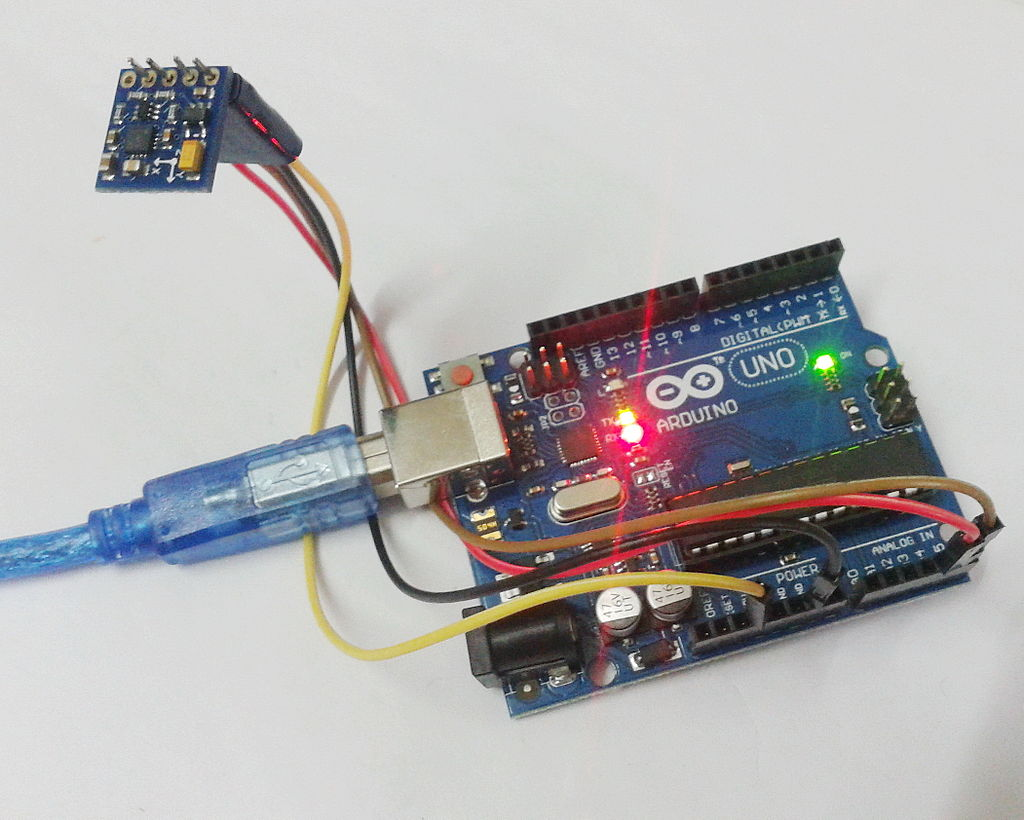
\includegraphics[height=0.4\textheight]{images/IoT-Sensor.jpg}
	\caption[Bild eines IoT-Sensors.]{Bild eines IoT-Sensors.
		Dieser besteht aus dem Mikrocontroller Arduino Uno, welcher die Steuerung übernimmt, und einem Gyroskop als Sensor, welcher an den Mikrocontroller angeschlossen ist.
		Er weist einige Schnittstellen wie Pins, USB und WLAN auf.\footnotemark
	}
	\label{pic:iotsensor}
\end{figure}

Als IoT-Sensoren werden autonome, netzwerkfähige Sensoren bezeichnet, wie in \cref{pic:iotsensor} zu sehen~\cite{IoTSensor}.
Ihr Aufbau ist, wie in der Abbildung zu sehen, simpel und besteht meist aus einem Mikrocontroller, der die Steuerung übernimmt, einem Sensor, der die Messung durchführt, einer Stromversorgung sowie einer Kommunikationsschnittstelle.
Es gibt verschiedene Arten von IoT-Sensoren, die in unterschiedlichen Bereichen wie der Industrie, der Landwirtschaft oder dem Garten eingesetzt werden.
Der Markt für IoT wächst stetig und es kommen immer neue Sensoren auf den Markt~\cite{IoTSensorenAbsatz}.

IoT-Sensoren können verschiedene Parameter messen, wie Temperatur, Luftfeuchtigkeit oder Bewegung.
Sie sind in der Lage, die gemessenen Daten an eine zentrale Stelle zu senden, wo sie ausgewertet werden können.
Dadurch können sie beispielsweise zur Überwachung bestimmter Parameter eingesetzt werden, wobei ein einzelner Sensor dabei meist nur einen Parameter misst.
Es gibt jedoch auch Sensoren, die mehrere Parameter messen können und dementsprechend flexibler einsetzbar sind.

IoT-Sensoren können sowohl fest installiert als auch mobil sein und außerdem können sie autonom arbeiten und benötigen keine manuelle Bedienung.
Dadurch können sie beispielsweise in schwer zugänglichen Bereichen eingesetzt werden.
Sie sind normalerweise stromsparend und können über lange Zeiträume betrieben werden, wodurch sie sich auch für den Einsatz in abgelegenen Gebieten eignen.
Außerdem sind sie meist kostengünstig und können in großen Stückzahlen eingesetzt werden.
Wie in \cref{pic:iotsensor} zu sehen, sind IoT-Sensoren einfach aufgebaut und können auch von Laien gebaut werden.

Gleichzeitig erfüllen die IoT-Sensoren allein nicht die Anforderungen an eine Automatisierung von Prozessen.
Sie können aber als Grundlage oder als Teil eines solchen Systems dienen und dabei die Rolle der Sensorik, nicht aber der Aktuatorik und Steuerung übernehmen.
Dies bietet einige Vorteile im Vergleich zu herkömmlichen Sensoren.
So müssen für eine größere Fläche keine Kabel durch den ganzen Garten gelegt werden, um Sensoren zu verbinden und gleichzeitig ist der Umbau leichter.
Auch wird durch die Autonomie der einzelnen Sensoren ein einzelner Ausfallpunkt umgangen.
Gleichzeitig ergeben sich einige Nachteile im Vergleich zu einfachen Sensoren, wie mehr Ausfallmöglichkeiten aufgrund der höheren Komplexität.
Außerdem sind die Kosten höher, da jeder Sensor einen eigenen Mikrocontroller, eine eigene Stromversorgung und Kommunikationsschnittstelle benötigt.
Zusammengefasst können IoT-Sensoren als Teil eines universellen Sensor- und Aktuatorsystems für Smart Gardening eingesetzt werden, indem sie die Rolle einiger Sensoren einnehmen, sie sind aber kein Ersatz für das Gesamtsystem.
\footnotetext{Bildquelle: Rahat, \href{https://creativecommons.org/licenses/by/4.0}{CC BY 4.0}, via Wikimedia Commons}



\section{Gateway}
\begin{figure}[!htb]
	\centering
	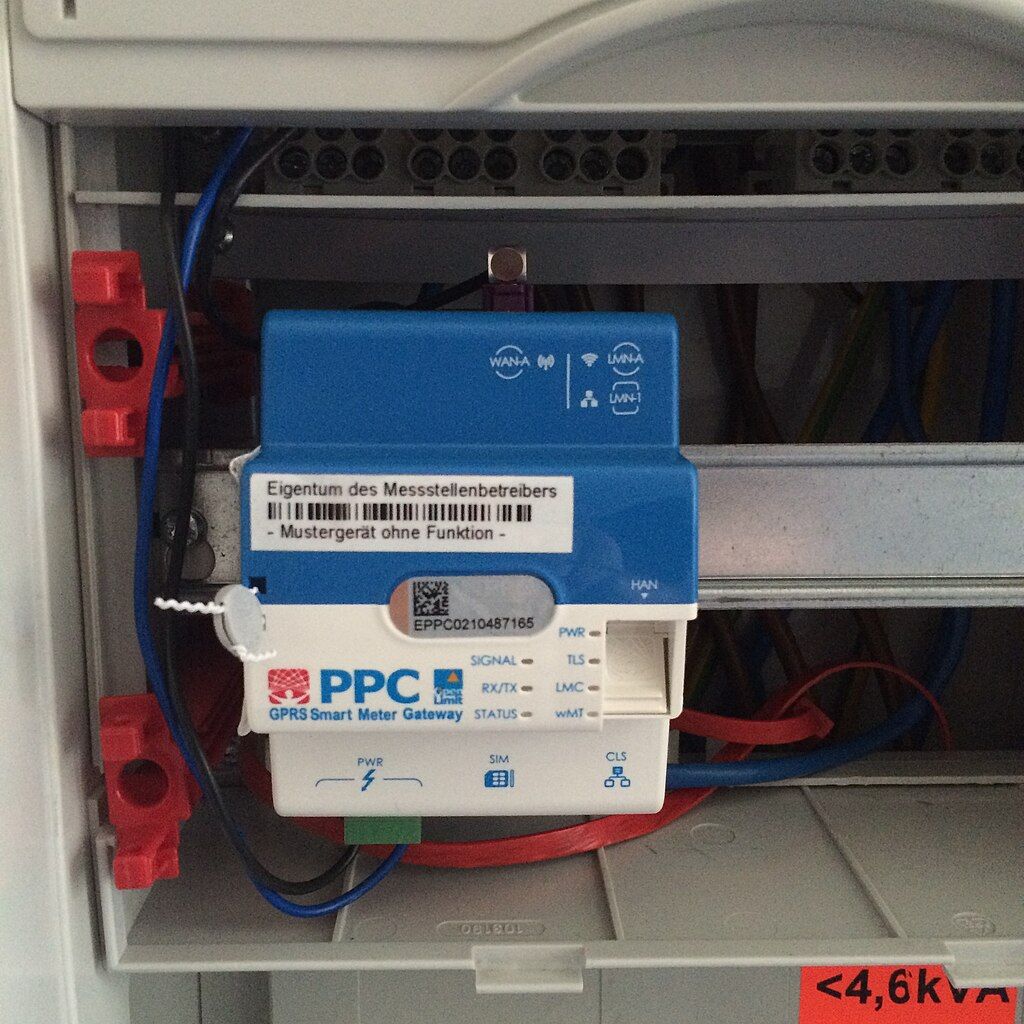
\includegraphics[height=0.4\textheight]{images/Gateway.jpg}
	\caption[Bild eines Smart-Meter-Gateways]{
		Bild eines Smart-Meter-Gateways, welches als Gateway für das lokale metrologische Netzwerk, ein Netz aus elektronischen Zählern wie Strom, Wasser, Gas und Wärme zu einem WAN und einem HAN dient~\cite{SmartMeterGateway}.\footnotemark
	}
	\label{pic:gateway}
\end{figure}
\footnotetext{Bildquelle: Pichiciago, \href{https://creativecommons.org/licenses/by-sa/4.0}{CC BY-SA 4.0}, via Wikimedia Commons}
In diesem Kontext bezeichnet ein Gateway eine Technologie, mit der Geräte ohne Internetfähigkeit internetfähig gemacht werden können.
Gateways können beispielsweise für Industrieanlagen, Sensoren oder Aktuatorik eingesetzt werden und haben häufig die Form einer kleinen Box wie in \cref{pic:gateway} zu sehen.
Auch Sensornetze, also Verbunde aus untereinander kommunizierenden Sensorknoten, können über ein Gateway an das Internet angeschlossen werden.
Häufig sind in solchen Anlagen Schnittstellen für beispielsweise Modbus verfügbar, an die das Gateway angeschlossen werden kann.
So ist ein Zugriff auf Daten sowie einer Steuerung über das Netzwerk möglich, was ohne Gateway nur vor Ort möglich wäre.
Auch einfache Sensoren können auf diese Art ihre Daten dem Netzwerk zur Verfügung stellen.

Als rein unterstützende Technologie können Gateways den definierten Anforderungen nicht entsprechen, da sie weder die Sensorik noch die Aktuatorik darstellen.
Sie können dennoch ein wichtiger Bestandteil eines solchen Systems sein, da sie die Integration von Sensoren und Aktuatoren in das Netzwerk ermöglichen.
So können etwa einfache Sensoren zu IoT-Sensoren aufgerüstet und Aktuatorik internetfähig gemacht werden, was eine Flexibilität im Aufbau des Systems ermöglicht.

Zusammengefasst können Gateways ein Bestandteil eines universellen Sensor- und Aktuatorsystems für Smart Gardening darstellen, indem sie Sensoren oder Aktuatoren an das System anschließen.
Sie sind jedoch nur unterstützende Technologie und können die Anforderungen nicht erfüllen.



\section{Messkoffer}
Als Messkoffer werden simple Koffer bezeichnet, die verschiedene Messgeräte enthalten.
Dabei kann es sich um einfache Multimeter, aber auch um komplexere Geräte handeln.
Meist sind diese Koffer beim Verkauf mit einer bestimmten Auswahl an Geräten bestückt, die von Handwerkern oder Technikern verwendet werden, um verschiedene Messungen durchzuführen.
Solche Messkoffer existieren auch für den Gartenbereich und können den Gärtner mobil bei der Arbeit unterstützen.
Sie sind jedoch nicht autonom, sondern müssen vom Nutzer bedient und die anfallenden Daten müssen durch den Nutzer manuell ausgewertet werden.
Auch Benachrichtigungen bei bestimmten Ereignissen wie bestimmten Temperaturschwellenwerten sind nicht möglich.
Aus diesen Gründen sind sie nicht für die Automatisierung von Prozessen geeignet.

\begin{figure}[!htb]
	\centering
	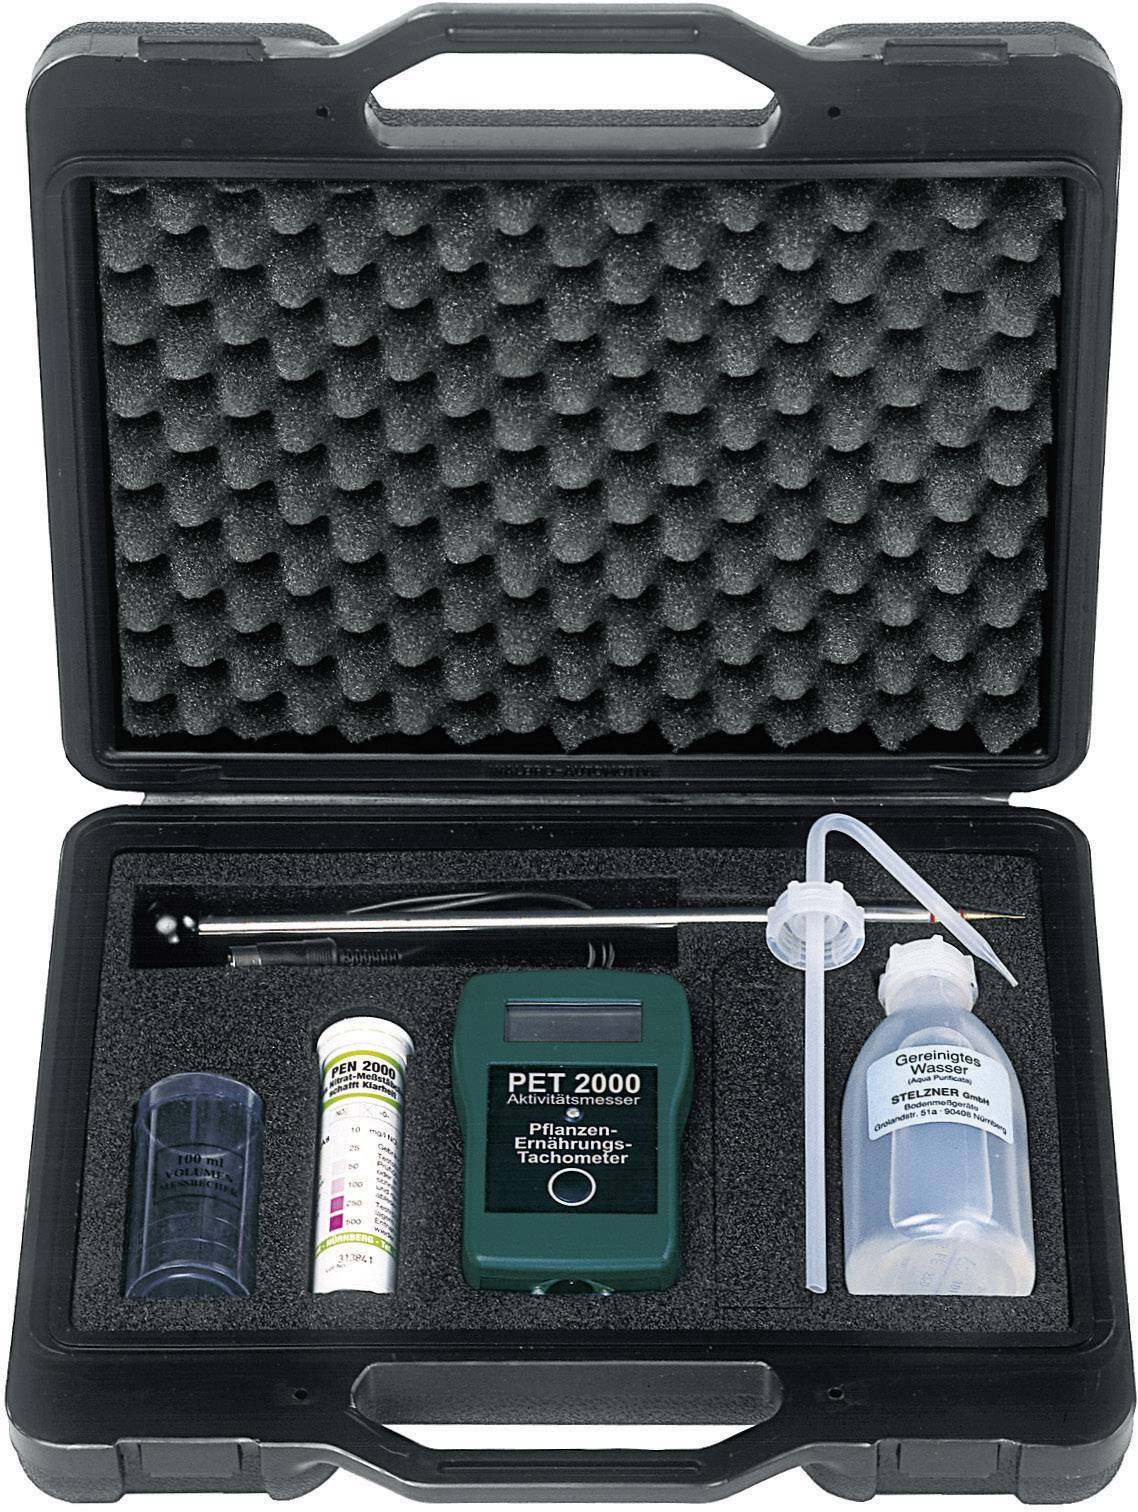
\includegraphics[width=0.4\textwidth]{images/Messkoffer.jpg}
	\caption[Bild eines Stelzner Aktivitätsmesskoffer PET 2000.]{
		Bild eines Stelzner Aktivitätsmesskoffer PET 2000.
		Dieser beinhaltet unter anderem einen Aktivitätsmesser PET 2000, Nitrat-Messstäbchen, Behälter und eine Flasche mit entinonisiertem Wasser.\footnotemark}
	\label{pic:messkoffer}
\end{figure}

\footnotetext{\href{https://asset.conrad.com/media10/isa/160267/c1/-/de/101879_BB_00_FB/image.jpg}{Bildquelle: Stelzner Aktivitätsmesskoffer PET 2000}}

Ein Beispiel dafür ist der Stelzner Aktivitätsmesskoffer PET 2000~\cite{Stelzner}, dessen Einsatzgebiet hauptsächlich der Gartenbau ist.
Dieser Koffer enthält, wie in \cref{pic:messkoffer} zu sehen, das Messgerät PET 2000 zur Bestimmung der im Boden gelösten Nährsalze, sowie Nitratmessstäbchen und weitere unterstützende Materialien.
Auf Basis dieser Messungen kann der Gärtner entscheiden, ob und wie gedüngt werden muss.
Somit deckt der Koffer einen Anwendungsfall ab, nämlich die Düngung.
Da aber sowohl Messung als auch Entscheidung über die Düngung manuell durch den Gärtner durchgeführt werden muss, decken solche Messkoffer die Anforderungen nicht ab.
Zusammengefasst sind Messkoffer nur teilweise Smart Gardening geeignet, da sie den Gärtner zwar in bestimmten Aufgaben unterstützen, jedoch keine Automatisierung von Messungen und Prozessen ermöglichen.




\section{Sensor-Hub}
Ein Sensor-Hub ist ein Gerät, das verschiedene Anschlüsse aufweist und somit mit unterschiedlichen Sensoren und Geräten verbunden werden kann.
Es kann sowohl mobil und somit an vielen Orten einsetzbar sein als auch fest installierbar.
Gleichzeitig ist es autonom, sodass es auch ohne manuelle Bedienung arbeiten kann.
Diese Technologie kann in verschiedenen Bereichen eingesetzt werden, wie in der Industrie, der Landwirtschaft oder im Gartenbau.
Dabei kann es sowohl für einfache Messungen als auch für komplexere Messungen eingesetzt werden, wobei komplex bedeutet, dass mehrere Messungen zu einem neuen Wert kombiniert werden.
Das kann etwa die Kombination von Temperatur und Luftfeuchtigkeit sein, um den Belüftungsbedarf eines Raumes zu bestimmen oder die Kombination von mehreren Pegelmessungen in einer Regentonne, um die Restdauer der Bewässerung zu bestimmen.

\subsection{Universal Wireless Sensor Node}

\begin{figure}[!htb]
	\centering
	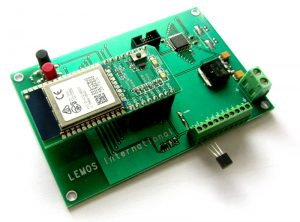
\includegraphics[width=0.5\textwidth]{images/UniversalWirelessSensorNode.jpg}
	\caption[Bild eines Universal Wireless Sensor Node.]{Bild eines Universal Wireless Sensor Node.\footnotemark}
	\label{pic:universal-sensor-node}
\end{figure}

\footnotetext{Bildquelle: \href{https://lemosint.com/wp-content/uploads/2019/04/UniversalWirelessSensorNode-300x222.jpg}{Universal Wireless Sensor Node}}

Der Universal Wireless Sensor Node von Lemos International Company Inc., wie in \cref{pic:universal-sensor-node} dargestellt~\cite{Universal}, basiert auf einem fortschrittlichen Mikrocontroller und ist in der Lage, eine Vielzahl von Sensoren für unterschiedliche Anwendungen zu integrieren.
Es unterstützt die Erfassung von Daten wie Temperatur, Luftfeuchtigkeit, Bewegungen und gefährlichen Gasen.
Dafür verfügt es über einige Protokolle zur Kommunikation, darunter I2C, SPI und asynchrone Protokolle.
Der Sensor Node kann mit verschiedenen Funkmodulen betrieben werden, die in energiesparenden, lizenzfreien Frequenzbereichen wie 433 MHz, 915 MHz und 2.4 GHz und dem amerikanischen Multi-Use Radio Service arbeiten.
Diese Flexibilität ermöglicht den Einsatz in zahlreichen Mess- und Steuerungsaufgaben, die für Smart Gardening relevant sind.
Gleichzeitig erfüllt der Universal Wireless Sensor Node die Anforderungen an ein universelles Sensor- und Aktuatorsystem für Smart Gardening nur teilweise.
Er kann zwar eine Vielzahl von Sensoren integrieren und die Daten an eine zentrale Stelle senden, jedoch fehlt die Aktuatorik und Steuerung.

\subsection{Loggito Logger}

\begin{figure}[!htb]
	\centering
	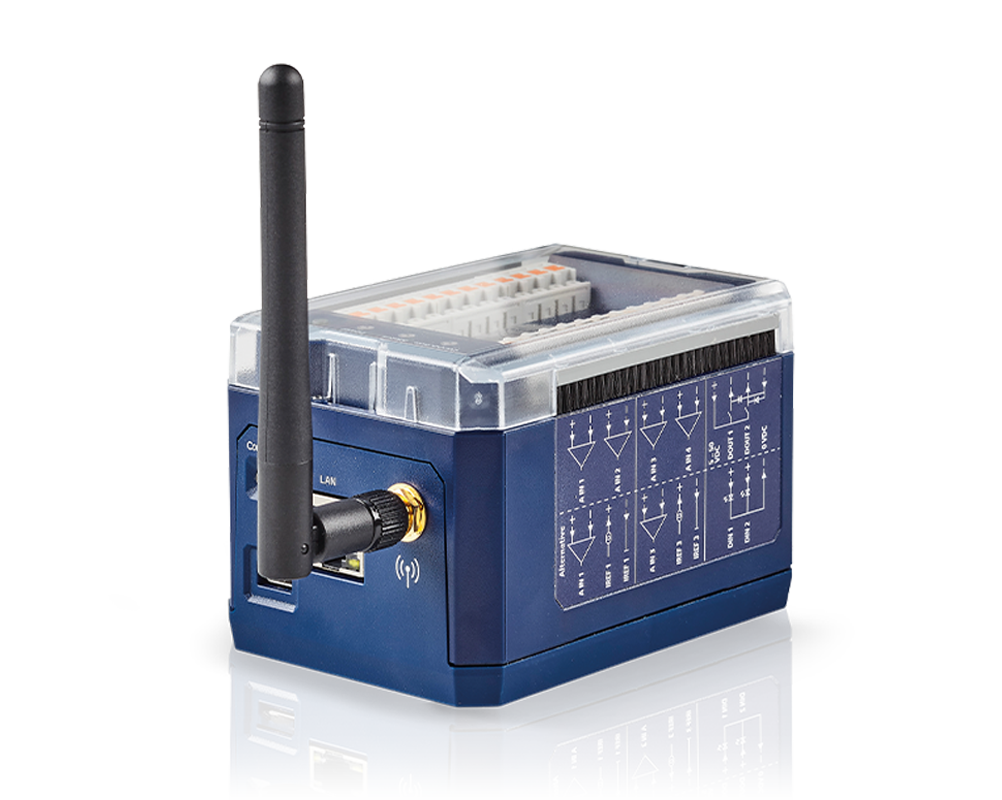
\includegraphics[height=0.3\textheight]{images/Loggito.png}
	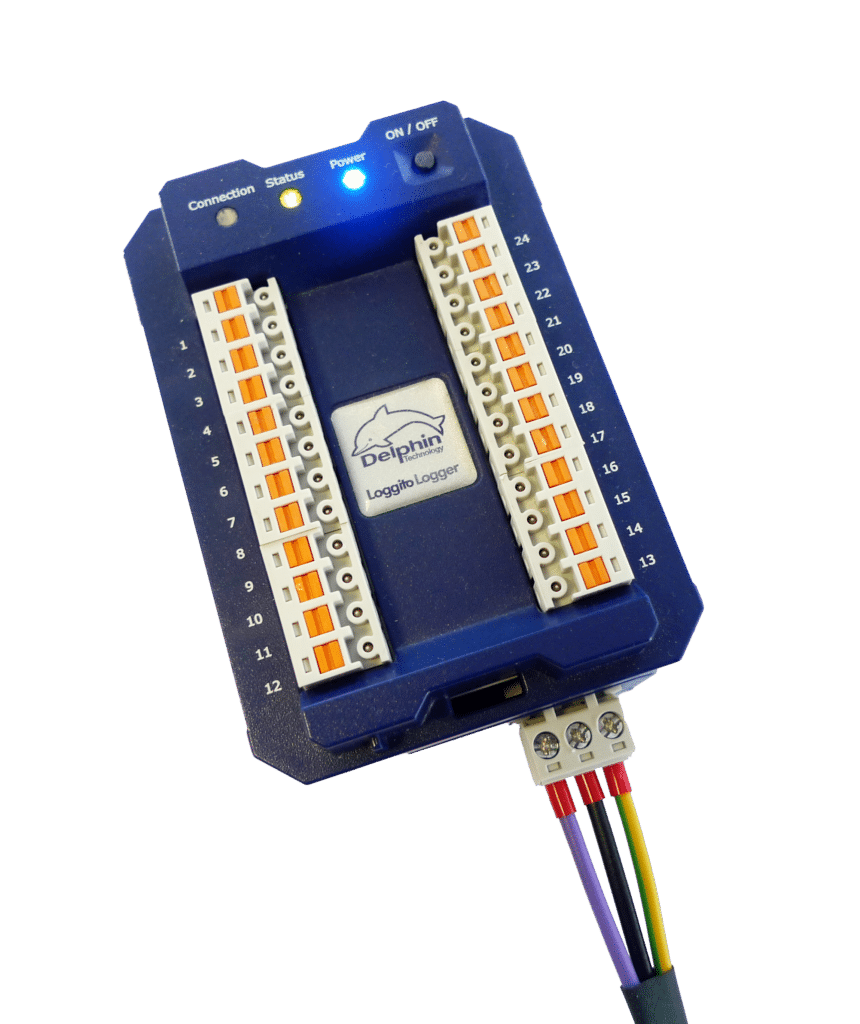
\includegraphics[height=0.3\textheight]{images/Loggito-von-oben.png}
	\caption[Bilder eines Loggito Logger von Delphin Technology.]{
		Bilder eines Loggito Logger von Delphin Technology von der Seite und von oben.
		Dabei ist der modulare Steckplatz mit 24 Eingängen sichtbar, die mit verschiedenen Modulen bestückt werden können.
		Außerdem zeigt das linke Bild eine Vielzahl von Schnittstellen, wie USB, Ethernet und WLAN.\footnotemark
	}
	\label{pic:loggito}
\end{figure}

\footnotetext{Bildquelle: \href{https://www.delphin.de/}{Delphin Technology}}

Der Datenlogger Loggito Logger von Delphin Technology~\cite{LoggitoLogger} ist wie rechts in \cref{pic:loggito} zu sehen, mit einem modularen Steckplatzsystem mit 24 Eingängen ausgestattet, sodass an diesen viele Sensoren angeschlossen werden können.
Diese einzelnen Steckplätze können mit unterschiedlichen Modulen bestückt werden, die verschiedene Schnittstellen aufweisen.
Auf der linken Seite sind weitere Schnittstellen sichtbar, unter anderem USB, Ethernet und eine Antenne für WLAN.
Somit kann der Loggito Logger mit verschiedenen Sensoren und Geräten verbunden werden und die Daten an eine zentrale Stelle senden.
In anderen Ausführungen werden auch andere Schnittstellen wie OPC UA, CAN-Bus, Profibus und RS 232/485 mit Modbus unterstützt.
Er weist einen IP67-Schutz auf, sodass er auch im Freien eingesetzt werden kann~\cite{LoggitoIP67}.
Weiterhin ist er autonom und kann auch ohne manuelle Bedienung arbeiten und erfüllt somit Teile der Anforderungen.
Gleichzeitig ist zwar eine komplexe Kombination von Messungen zu neuen Werten möglich, jedoch keine Regeldefinition und keine Steuerung.
Auch ist der Loggito Logger nicht stromsparend konzipiert, sodass ein Betrieb ohne externe Stromversorgung und somit in vielen Gärten eine Herausforderung ist.

\subsection{SCAMPI}
\emph{Sensor Configuration and Aggregation Middleware for Multi Platform Interchange} (SCAMPI) ist ein Middleware-System, das die Aggregation von Sensordaten aus heterogenen Quellen ermöglicht und in der Cloud liegt~\cite{SCAMPI}.
Dazu gehört außerdem ein regelbasiertes System zur Erzeugung virtueller Sensoren, das aus den aggregierten Daten höherwertige Informationen generieren.
Diese virtuellen Sensoren können dann wiederum als Eingabe für andere virtuelle Sensoren dienen, sodass komplexe Regelwerke erstellt werden können.
Gleichzeitig erfolgt der Zugriff auf sowohl virtuelle als auch physische Sensoren über eine einheitliche Schnittstelle, sodass die Integration von Sensoren vereinfacht wird.
Die Sensordaten können über ein Dashboard visualisiert und kombiniert werden zu Digital Twins, die den Zustand eines realen Objekts abbilden.
Als Middleware-System in der Cloud ist SCAMPI jedoch nicht nah an den Sensoren und somit müssen einfache Sensoren erst an ein Gateway angeschlossen werden, um sie in SCAMPI zu integrieren.
Weiterhin ermöglicht SCAMPI selbst keine Steuerung von Aktuatorik, sondern nur die Aggregation und Verarbeitung von Sensordaten.
Dementsprechend erfüllt SCAMPI die Anforderungen an ein universelles Sensor- und Aktuatorsystem für Smart Gardening nur teilweise.
Gleichzeitig kann SCAMPI als Grundlage für ein solches System dienen, da es die Aggregation und Verarbeitung von Sensordaten ermöglicht.

\subsection{Smart Garden Hub von GreenIQ}
Der Smart Garden Hub von GreenIQ ist ein mittlerweile eingestelltes autonomes Bewässerungssystem, das auf Wettervorhersagen und Sensoren basierend die Bewässerung bedarfsgerecht steuern kann~\cite{GreenIQ}.
Hierbei geht der Hub etwas weiter als ein reiner Sensor-Hub durch die Integration von Aktuatoren, die die Bewässerung steuern.
Als Sensoren konnten bestimmte IoT-Sensoren anderer Hersteller angeschlossen werden, die die Daten an den Smart Garden Hub senden.
Dazu gehören Wetterstationen, Regenmesser, Sonnenstandmesser und Feuchtigkeitssensoren.
Hierbei können jedoch nur IP-basierte Sensoren angeschlossen werden, was die Flexibilität einschränkt.
Dabei ist der Smart Garden Hub nur für die Bewässerung ausgelegt und kann keine anderen Aktuatoren steuern, deckt also nur einen Teil der Anwendungsfälle ab.
Weiterhin sind die Konfigurationsmöglichkeiten eingeschränkt, sodass individuelle Anpassungen schwierig sind.
Dementsprechend ist der Smart Garden Hub nur für spezifische Anwendungsfälle geeignet und kann die Anforderungen an ein universelles Sensor- und Aktuatorsystem für Smart Gardening nicht vollständig erfüllen.

\subsection{Zusammenfassung der Sensor Hubs}
Zusammengefasst ist ein Sensor-Hub ein vielseitiges Gerät, das verschiedene Sensoren und Geräte miteinander verbindet, um sowohl einfache als auch komplexe Messungen autonom durchzuführen.
Der Loggito Logger von Delphin Technology ist ein robustes und modulares Gerät, das viele Sensoren integrieren kann und mit verschiedenen Schnittstellen ausgestattet ist.
Der Universal Wireless Sensor Node von Lemos International kann eine breite Palette an Sensordaten erfassen, verarbeiten und an eine zentrale Stelle senden.
SCAMPI ist eine Middleware zur Aggregation und Verarbeitung von Sensordaten, dient also als Hub, jedoch ohne direkte Steuerungsmöglichkeiten.
Der Smart Garden Hub von GreenIQ ist auf die Bewässerung spezialisiert und integriert nur bestimmte IoT-Sensoren.
Gleichzeitig ermöglicht er eine Steuerung der Bewässerung, welche die anderen Hubs nicht bieten.
Insgesamt fehlt es den meisten Sensor-Hubs an umfassender Steuerungsintegration für ein universelles Sensor- und Aktuatorsystem für Smart Gardening.



\section{Industrial Remote Monitoring (and Control)}
Industrial Remote Monitoring bezeichnet die Fernüberwachung von industriellen Anlagen und Prozessen.
Dies kann in verschiedenen Industrien eingesetzt werden.
Dazu gehören unter anderem das verarbeitende Gewerbe, die Landwirtschaft und Transportsysteme.
Diese Systeme bestehen aus verteilter Sensorik, die die Daten an eine cloudbasierte Softwareplattform senden~\cite{IdustrialRemoteMonitoring}, wobei es sich bei der Sensorik um IoT-Sensoren handeln kann.
Hierbei werden die Daten aggregiert verarbeitet und auf Basis dieser Verarbeitung können auch Benachrichtigungen generiert werden.
Dieses Systemkonzept entspricht grob dem Sensor- und Aktuatorsystem für Smart Gardening, wobei die Aktuatorik fehlt.
Gleichzeitig bedeutet der Fokus auf die Industrie, dass solche Systeme entsprechend bepreist sind.
Auch sind sie für industrielle Skalierung ausgelegt, was häufig viel Overhead bedeutet und für einen einfachen Garten nicht verhältnismäßig ist.

\subsection{Journeo}
Das von der britischen Firma Journeo entwickelte Fernüberwachungssystem wird es hauptsächlich im öffentlichen Nah-, Bahn- und Warenverkehr und ermöglicht die Einbindung vieler IoT-Sensoren und Kameras in ein System~\cite{Journeo}.
Gleichzeitig ermöglicht dieses System keine Steuerung, sondern nur eine Fernüberwachung und ist auch nicht an den Gartenbereich angepasst.
Außerdem handelt es sich um ein kommerzielles Produkt, das nicht an Privatpersonen vertrieben wird und entsprechend teuer ist.
Somit kann es die Anforderungen an ein universelles Sensor- und Aktuatorsystem für Smart Gardening nicht vollständig erfüllen.

\subsection{Jain Unity}
Eine Erweiterung von Industrial Remote Monitoring ist Industrial Remote Monitoring and Control, bei dem auch die Steuerung von Prozessen möglich ist.
Es ist also nicht nur eine Fernüberwachung möglich, sondern auch eine Steuerung, wodurch auch Aktuatorik betrieben werden kann.

Bei Jain Unity von Jain Irrigation handelt es sich um ein automatisches Bewässerungssystem für die Landwirtschaft, welches Messungen des Bodens mit Wetterdaten und Satellitenbildern kombiniert~\cite{Jain}.
Diese Daten werden von einem KI-System für Bewässerungsentscheidungen verwendet, welche automatisch durch Öffnung entsprechender Ventile umgesetzt werden.
Dieses spezifische System erfüllt einen Teil der Anwendungsfälle, nämlich die automatische Bewässerung.
Ein Smart Gardening System besteht aber nicht nur aus einer automatischen Bewässerung, sodass dieses System nicht alle Anwendungsfälle abdeckt und daher die Anforderungen nicht erfüllen kann.
Weiterhin ist das System nicht modular erweiterbar, sondern als Gesamtsystem konzipiert, was die Anpassung an individuelle Bedürfnisse erschwert.
Außerdem ist das System auf die kommerzielle Landwirtschaft ausgelegt, was sich in der Preisgestaltung widerspiegelt und für den privaten Gartenbereich nicht geeignet ist.
Aus diesen Gründen ist das System zwar für einen spezifischen Anwendungsfall geeignet, aber nicht als ein universelles Sensor- und Aktuatorsystem für Smart Gardening.

\subsection{Zusammenfassung von Industrial Remote Monitoring (and Control)}
Zusammengefasst bezieht sich Industrial Remote Monitoring auf die Fernüberwachung industrieller Anlagen und Prozesse in verschiedenen Branchen wie dem verarbeitenden Gewerbe, der Landwirtschaft und dem Transportwesen.
Diese Systeme nutzen verteilte IoT-Sensoren, die Daten an eine meist cloudbasierte Plattform senden, wo sie verarbeitet und beispielsweise zur Generierung von Benachrichtigungen verwendet werden.
Ein Beispiel ist das Fernüberwachungssystem der Firma Journeo, das IoT-Sensoren und Kameras im Verkehrsbereich integriert, jedoch keine Steuerung ermöglicht und nicht auf den Gartenbereich zugeschnitten ist.

Eine Erweiterung dieses Konzepts ist Industrial Remote Monitoring and Control, das auch die Steuerung von Prozessen umfasst.
Ein Beispiel hierfür ist das automatische Bewässerungssystem Jain Unity, das Bodendaten, Wetterdaten und Satellitenbilder kombiniert.
Darauf basierend werden durch ein KI-System bewässerungsbezogene Entscheidungen getroffen und entsprechende Ventile automatisch gesteuert.
Obwohl dieses System für spezifische Anwendungsfälle wie die automatische Bewässerung geeignet ist, erfüllt es nicht die umfassenden Anforderungen eines modularen und universellen Sensor- und Aktuatorsystems für Smart Gardening, da es nicht modular erweiterbar ist und nur eingeschränkte Anpassungsmöglichkeiten bietet.
Da Industrial Remote Monitoring and Control aber sowohl Sensorik als auch Aktuatorik unterstützt, kann das angestrebte Sensor- und Aktuatorsystem für Smart Gardening als Remote Monitoring and Control bezeichnet werden, wobei explizit der Fokus auf den Gartenbereich und nicht auf die Industrie gelegt wird.
Gleichzeitig decken existierende Lösungen nicht alle Anwendungsfälle und Anforderungen ab.

\section{Gegenüberstellung}
In diesem Abschnitt werden die verschiedenen Systeme gegenübergestellt und anhand der funktionalen und nicht funktionalen Anforderungen bewertet.
Dafür werden die Anforderungen verwendet, die im vorherigen Kapitel aufgestellt und priorisiert wurden.

\begin{table}[!htb]
	\centering
	\caption[Konzepte und Beispiele: funktionale Anforderungen.]{
		Darstellung, welche Konzepte und Beispiele welche funktionalen Anforderungen erfüllen.
		In den Zeilen sind die verschiedenen Konzepte und Beispiele aufgeführt, in den Spalten die funktionalen Anforderungen.
		Hierbei sind die Konzepte hervorgehoben und die Beispiele sind jeweils unter den Konzepten normal aufgeführt.
		Die von einem Konzept beziehungsweise einer Realisierung erfüllten Anforderungen sind mit einem Häkchen markiert.
		Nicht erfüllte Anforderungen werden durch ein Kreuz markiert.
	}\label{tab:sdt-funkt-anforderungen}
	\begin{tabular}{llllllllll}
		\rot[\tabellenwinkel]{					} &
		\rot[\tabellenwinkel]{Messung			} &
		\rot[\tabellenwinkel]{Konfiguration		} &
		\rot[\tabellenwinkel]{Regeldefinition	} &
		\rot[\tabellenwinkel]{Dashboard			} &
		\rot[\tabellenwinkel]{Steuerung			} &
		\rot[\tabellenwinkel]{Autonomer Betrieb	} &
		\rot[\tabellenwinkel]{Benachrichtigung	} \\\hline
		\emph{IoT-Sensor}								& \OK & \NO & \NO & \NO & \NO & \OK & \NO \\
		\emph{Gateway}									& \NO & \NO & \NO & \NO & \NO & \OK & \NO \\
		\emph{Messkoffer}								& \OK & \NO & \NO & \NO & \NO & \NO & \NO \\
		Aktivitätsmesskoffer PET 2000					& \OK & \NO & \NO & \NO & \NO & \NO & \NO \\
		\emph{Sensor-Hub}								& \OK & \OK & \NO & \NO & \NO & \OK & \NO \\
		Universal Wireless Sensor Node					& \OK & \OK & \NO & \NO & \NO & \OK & \NO \\
		Loggito Logger									& \OK & \OK & \NO & \OK & \NO & \OK & \NO \\
		SCAMPI											& \OK & \OK & \OK & \OK & \NO & \OK & \NO \\
		Smart Garden Hub von GreenIQ					& \OK & \NO & \NO & \OK & \OK & \OK & \OK \\
		\emph{Industrial Remote Monitoring}				& \OK & \OK & \OK & \OK & \NO & \OK & \OK \\
		Journeo											& \OK & \OK & \NO & \OK & \NO & \OK & \OK \\
		\emph{Industrial Remote Monitoring and Control}	& \OK & \OK & \OK & \OK & \OK & \OK & \OK \\
		Jain Unity										& \OK & \NO & \NO & \OK & \OK & \OK & \OK \\
	\end{tabular}
\end{table}

Zunächst werden die funktionalen Anforderungen betrachtet, die in \cref{tab:sdt-funkt-anforderungen} dargestellt sind.
In der Tabelle sind dabei sowohl die jeweiligen Konzepte als auch Beispiele aufgeführt, wenn solche analysiert wurden.
Dabei ist zu beachten, dass die Zuordnung der Beispiele zu den Konzepten auf Basis der Beschreibung erfolgt und somit nicht immer die gleichen Anforderungen erfüllt werden.
Als Erstes fällt auf, dass kein Beispiel und nur ein Konzept, nämlich das Industrial Remote Monitoring and Control, alle funktionalen Anforderungen erfüllt.
Der IoT-Sensor und das Gateway erfüllen nur wenige Anforderungen, können aber in einem System als Grundlage für die Sensorik eingesetzt werden.
Dies steht im Gegensatz zu den Messkoffern, die nur durch manuelle Bedienung arbeiten und daher nicht in einem solchen System eingesetzt werden können.
Das Konzept des Sensor-Hubs erfüllt mehr Anforderungen, wichtige Anforderungen wie die Steuerung und Regeldefinition fehlen jedoch weiterhin.
Je nach Sensor-Hub ist eine Erweiterung potenziell möglich, sodass sie als Teil eines Smart Gardening Systems eingesetzt werden können.
Gleichzeitig erfüllen die einzelnen Beispiele für Sensor-Hubs meist weitere Anforderungen, wie SCAMPI, das auch Regeldefinitionen ermöglicht oder der Smart Garden Hub von GreenIQ welcher auch die Steuerung der Bewässerung ermöglicht.
Das Industrial Remote Monitoring erfüllt bereits die meisten funktionalen Anforderungen, jedoch fehlt die Steuerung und Journeo fehlt zusätzlich die Anforderung der Regeldefinition.
Das Industrial Remote Monitoring and Control erfüllt alle funktionalen Anforderungen, jedoch ist Jain Unity nicht modular konfigurierbar und es ermöglicht keine Regeldefinition, wodurch es nicht universell einsetzbar ist.

\begin{table}[!htb]
	\centering
	\caption[Konzepte und Beispiele: nicht funktionale Anforderungen.]{
		Darstellung, welche Konzepte und Beispiele die nicht funktionalen Anforderungen erfüllen.
		In den Zeilen sind die verschiedenen Konzepte und Beispiele aufgeführt, in den Spalten die nicht funktionalen Anforderungen.
		Die von einem Konzept / einer Realisierung erfüllten Anforderungen sind mit einem Häkchen markiert.
		In einigen Fällen ist die Erfüllung einer Anforderung nicht eindeutig, in diesen Fällen ist ein Fragezeichen markiert.
		Und in einigen Fällen ist die Anforderung nicht zutreffend, in diesen Fällen ist ein Schrägstrich markiert.
		Nicht erfüllte Anforderungen werden durch ein Kreuz markiert.
	}\label{tab:sdt-non-funkt-anforderungen}
	\begin{tabular}{lllllllllll}
		\rot[\tabellenwinkel]{						} &
		\rot[\tabellenwinkel]{Preis					} &
		\rot[\tabellenwinkel]{Elementschutz			} &
		\rot[\tabellenwinkel]{Nutzerfreundlichkeit	} &
		\rot[\tabellenwinkel]{Sicherheit			} &
		\rot[\tabellenwinkel]{Energieverbrauch		} &
		\rot[\tabellenwinkel]{Verfügbarkeit			} &
		\rot[\tabellenwinkel]{Wartbarkeit			} &
		\rot[\tabellenwinkel]{Unauffälligkeit		} \\\hline
		Aktivitätsmesskoffer							& \OK & \OK & \OK & \OK & \OK & \OK & \OK & \OK \\
		Loggito Logger									& \UN & \OK & \OK & \OK & \NO & \OK & \OK & \NO \\
		Universal Wireless Sensor Node					& \OK & \NO & \NO & \UN & \OK & \OK & \OK & \OK \\
		SCAMPI											& \OK & \NA & \OK & \OK & \NA & \OK & \OK & \NA \\
		Smart Garden Hub von GreenIQ					& \OK & \OK & \OK & \OK & \OK & \OK & \UN & \OK \\
		Journeo											& \NO & \NA & \UN & \OK & \NA & \OK & \UN & \NA \\
		Jain Unity										& \NO & \OK & \UN & \OK & \NO & \OK & \UN & \NO \\
	\end{tabular}
\end{table}

Im Folgenden werden die nicht funktionalen Anforderungen betrachtet, die in \cref{tab:sdt-non-funkt-anforderungen} dargestellt sind.
Wichtig zu beachten ist hierbei, dass hier nur die Beispiele betrachtet werden, da diese mehr als bei den funktionalen Anforderungen eine Sache der Umsetzung sind.
So definiert das Konzept des Industrial Remote Monitoring keine notwendige IP-Schutzart, diese hängt vom Umfeld des konkreten Systems ab.
Ein solches System in einer Industrieanlage ist beispielsweise anderen Bedingungen ausgesetzt als ein System in der Landwirtschaft.
Auch für die einzelnen Beispiele sind nicht alle Anforderungen direkt anwendbar.
So ist der Elementschutz für SCAMPI nicht definierbar, da es sich um eine Cloud-basierte Middleware handelt und die genutzten Sensoren nicht genauer spezifiziert sind.
Weiterhin ist die Quellenlage für einige Anforderungen bei den Beispielen nicht eindeutig, sodass diese mit einem Fragezeichen markiert sind.
Insgesamt fällt auf, dass die meisten Anforderungen für die meisten Beispiele erfüllt oder nicht anwendbar sind.

Zusammengefasst werden die funktionalen Anforderungen von keinem Beispiel vollständig erfüllt und die Beispiele, die nah herankommen, erfüllen nicht alle nicht funktionalen Anforderungen.
Gleichzeit erfüllt nur eines der Konzepte alle funktionalen Anforderungen, nämlich das Industrial Remote Monitoring and Control.
Daher ist es sinnvoll, ein eigenes System zu entwickeln, das die Anforderungen erfüllt, welches sich am Konzept des Industrial Remote Monitoring and Control orientiert und dabei den Fokus auf den Gartenbereich statt der Industrie legt.


\section{Zusammenfassung des Stands der Technik}
In diesem Kapitel wurde der Stand der Technik analysiert, der potenziell für ein universelles Sensor- und Aktuatorsystem für Smart Gardening relevant ist, und mit den Anforderungen für dieses System verglichen.
Als Konzepte wurden IoT-Sensoren, Gateways, Messkoffer, Sensor-Hubs und Industrial Remote Monitoring (and Control) betrachtet.
IoT-Sensoren und Gateways sind als Grundlage für die Sensorik eines solchen Systems geeignet, können jedoch nicht die Systemrolle übernehmen.
Messkoffer sind für Smart Gardening nicht geeignet, da sie manuell bedient werden müssen und keine Automatisierung ermöglichen.
Sensor-Hubs können als Grundlage für das System dienen, sie erfüllen jedoch die meisten Anforderungen nicht, insbesondere die Steuerung.
Gleiches gilt für die Sensor-Hubs Beispiele, welche zwar meist mehr Anforderungen erfüllen, jedoch weiterhin nicht alle.
Industrial Remote Monitoring and Control erfüllt alle funktionalen Anforderungen, dies gilt jedoch nicht für Jain Unity.
Dieses Beispiel erfüllt auch die nicht funktionalen Anforderungen nicht vollständig.
Insgesamt erfüllt kein Beispiel alle funktionalen und nicht funktionalen Anforderungen, sodass ein eigenes System entwickelt werden muss, das die Anforderungen erfüllt.
Im folgenden Kapitel wird ein Konzept für ein universelles Sensor- und Aktuatorsystem für Smart Gardening vorgestellt, das die Anforderungen erfüllt und auf den Erkenntnissen des Standes der Technik basiert.